\documentclass{standalone}
\usepackage{tikz}
\usetikzlibrary{patterns, positioning}

\begin{document}
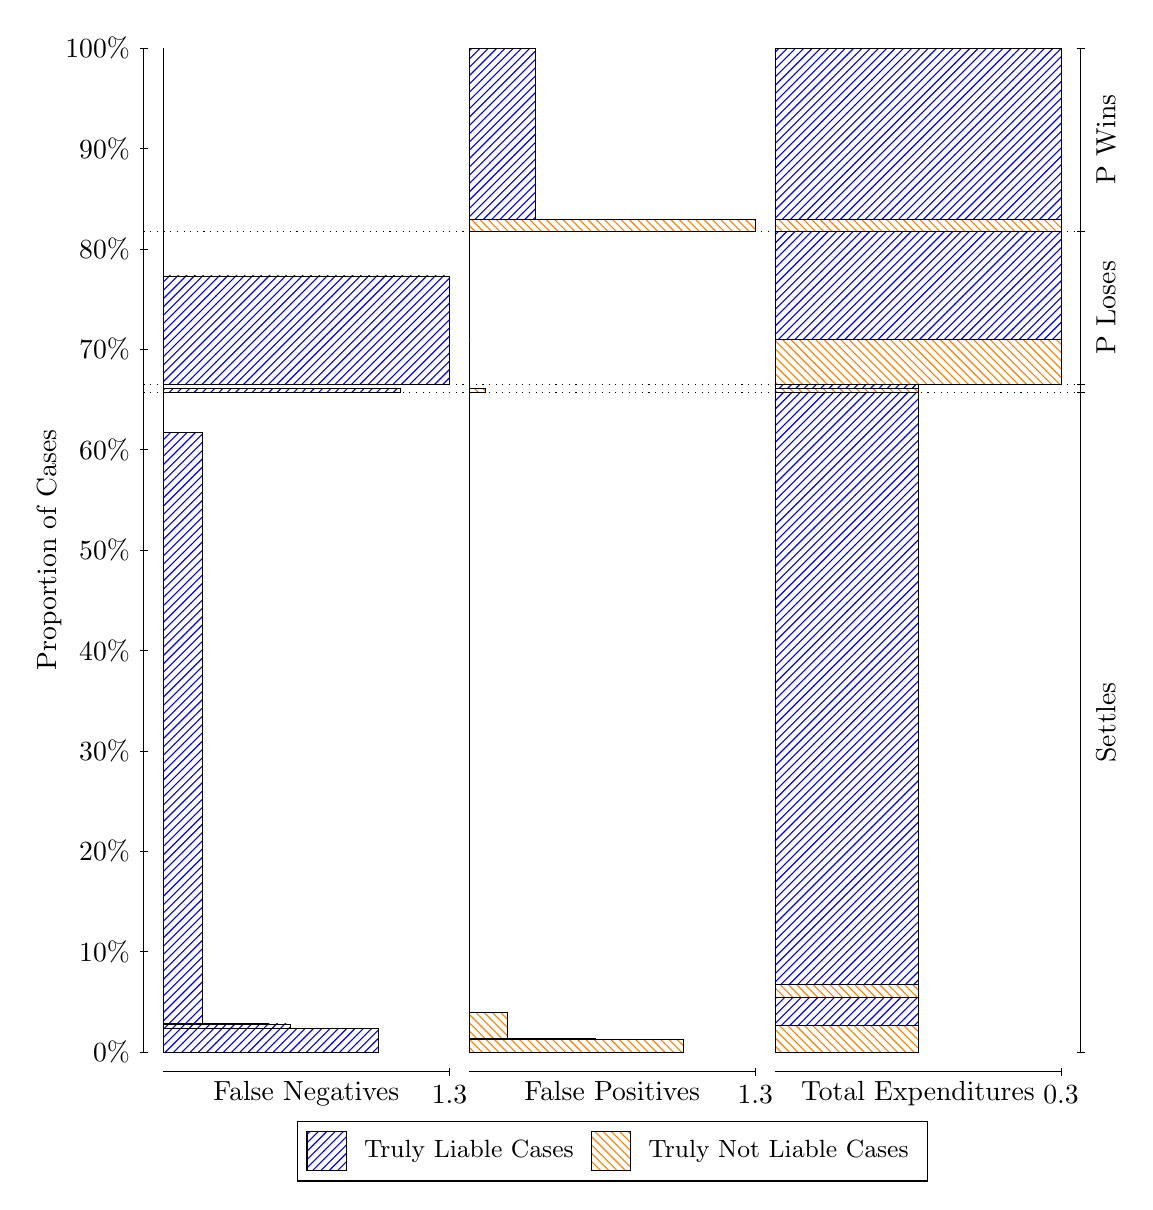
\begin{tikzpicture}
\draw[black, very thin] (1.5,1.75) -- (1.5,14.5);
\node[rotate=90, anchor=center] at (0.3, 8.125) {Proportion of Cases};
\draw[black, very thin] (1.45,1.75) -- (1.55,1.75);
\node[anchor=east] at (1.45, 1.75) {0\%};
\draw[black, very thin] (1.45,3.025) -- (1.55,3.025);
\node[anchor=east] at (1.45, 3.025) {10\%};
\draw[black, very thin] (1.45,4.3) -- (1.55,4.3);
\node[anchor=east] at (1.45, 4.3) {20\%};
\draw[black, very thin] (1.45,5.575) -- (1.55,5.575);
\node[anchor=east] at (1.45, 5.575) {30\%};
\draw[black, very thin] (1.45,6.85) -- (1.55,6.85);
\node[anchor=east] at (1.45, 6.85) {40\%};
\draw[black, very thin] (1.45,8.125) -- (1.55,8.125);
\node[anchor=east] at (1.45, 8.125) {50\%};
\draw[black, very thin] (1.45,9.4) -- (1.55,9.4);
\node[anchor=east] at (1.45, 9.4) {60\%};
\draw[black, very thin] (1.45,10.675) -- (1.55,10.675);
\node[anchor=east] at (1.45, 10.675) {70\%};
\draw[black, very thin] (1.45,11.95) -- (1.55,11.95);
\node[anchor=east] at (1.45, 11.95) {80\%};
\draw[black, very thin] (1.45,13.225) -- (1.55,13.225);
\node[anchor=east] at (1.45, 13.225) {90\%};
\draw[black, very thin] (1.45,14.5) -- (1.55,14.5);
\node[anchor=east] at (1.45, 14.5) {100\%};

\draw[black, very thin] (13.4,1.75) -- (13.4,14.5);
\draw[black, very thin] (13.35,1.75) -- (13.45,1.75);
\node[anchor=west] at (13.35, 1.75) {};
\draw[black, very thin] (13.35,10.122) -- (13.45,10.122);
\node[anchor=west] at (13.35, 10.122) {};
\draw[black, very thin] (13.35,10.23) -- (13.45,10.23);
\node[anchor=west] at (13.35, 10.23) {};
\draw[black, very thin] (13.35,12.174) -- (13.45,12.174);
\node[anchor=west] at (13.35, 12.174) {};
\draw[black, very thin] (13.35,14.5) -- (13.45,14.5);
\node[anchor=west] at (13.35, 14.5) {};

\draw[black, very thin, pattern color=blue, pattern=north east lines] (1.75,1.75) rectangle (4.475,2.052);
\draw[black, very thin, pattern color=blue, pattern=north east lines] (1.75,2.052) rectangle (3.3571,2.1057);
\draw[black, very thin, pattern color=blue, pattern=north east lines] (1.75,2.1057) rectangle (3.0776,2.109);
\draw[black, very thin, pattern color=blue, pattern=north east lines] (1.75,2.109) rectangle (2.7981,2.1125);
\draw[black, very thin, pattern color=blue, pattern=north east lines] (1.75,2.1125) rectangle (2.5186,2.1161);
\draw[black, very thin, pattern color=blue, pattern=north east lines] (1.75,2.1161) rectangle (2.2391,9.6225);
\draw[black, very thin, pattern color=orange, pattern=north west lines] (1.75,9.6225) rectangle (1.75,10.122);
\draw[black, very thin, pattern color=blue, pattern=north east lines] (1.75,10.122) rectangle (4.7545,10.174);
\draw[black, very thin, pattern color=orange, pattern=north west lines] (1.75,10.174) rectangle (1.75,10.23);
\draw[black, very thin, pattern color=blue, pattern=north east lines] (1.75,10.23) rectangle (5.3833,11.606);
\draw[black, very thin, pattern color=orange, pattern=north west lines] (1.75,11.606) rectangle (1.75,12.174);
\draw[black, very thin, pattern color=orange, pattern=north west lines] (1.75,12.174) rectangle (1.75,12.326);
\draw[black, very thin, pattern color=blue, pattern=north east lines] (1.75,12.326) rectangle (1.75,14.5);
\draw[black, very thin, pattern color=orange, pattern=north west lines] (5.6333,1.75) rectangle (8.3583,1.9111);
\draw[black, very thin, pattern color=orange, pattern=north west lines] (5.6333,1.9111) rectangle (8.0788,1.9119);
\draw[black, very thin, pattern color=orange, pattern=north west lines] (5.6333,1.9119) rectangle (7.7994,1.9126);
\draw[black, very thin, pattern color=orange, pattern=north west lines] (5.6333,1.9126) rectangle (7.5199,1.9134);
\draw[black, very thin, pattern color=orange, pattern=north west lines] (5.6333,1.9134) rectangle (7.2404,1.9249);
\draw[black, very thin, pattern color=orange, pattern=north west lines] (5.6333,1.9249) rectangle (6.1224,2.2494);
\draw[black, very thin, pattern color=blue, pattern=north east lines] (5.6333,2.2494) rectangle (5.6333,10.122);
\draw[black, very thin, pattern color=orange, pattern=north west lines] (5.6333,10.122) rectangle (5.8429,10.178);
\draw[black, very thin, pattern color=blue, pattern=north east lines] (5.6333,10.178) rectangle (5.6333,10.23);
\draw[black, very thin, pattern color=orange, pattern=north west lines] (5.6333,10.23) rectangle (5.6333,10.798);
\draw[black, very thin, pattern color=blue, pattern=north east lines] (5.6333,10.798) rectangle (5.6333,12.174);
\draw[black, very thin, pattern color=orange, pattern=north west lines] (5.6333,12.174) rectangle (9.2667,12.326);
\draw[black, very thin, pattern color=blue, pattern=north east lines] (5.6333,12.326) rectangle (6.4718,14.5);
\draw[black, very thin, pattern color=orange, pattern=north west lines] (9.5167,1.75) rectangle (11.333,2.0861);
\draw[black, very thin, pattern color=blue, pattern=north east lines] (9.5167,2.0861) rectangle (11.333,2.4417);
\draw[black, very thin, pattern color=orange, pattern=north west lines] (9.5167,2.4417) rectangle (11.333,2.6051);
\draw[black, very thin, pattern color=blue, pattern=north east lines] (9.5167,2.6051) rectangle (11.333,10.122);
\draw[black, very thin, pattern color=orange, pattern=north west lines] (9.5167,10.122) rectangle (11.333,10.178);
\draw[black, very thin, pattern color=blue, pattern=north east lines] (9.5167,10.178) rectangle (11.333,10.23);
\draw[black, very thin, pattern color=orange, pattern=north west lines] (9.5167,10.23) rectangle (13.15,10.798);
\draw[black, very thin, pattern color=blue, pattern=north east lines] (9.5167,10.798) rectangle (13.15,12.174);
\draw[black, very thin, pattern color=orange, pattern=north west lines] (9.5167,12.174) rectangle (13.15,12.326);
\draw[black, very thin, pattern color=blue, pattern=north east lines] (9.5167,12.326) rectangle (13.15,14.5);
\draw[black, dotted] (1.5,10.122) -- (13.4,10.122);
\draw[black, dotted] (1.5,10.23) -- (13.4,10.23);
\draw[black, dotted] (1.5,12.174) -- (13.4,12.174);
\draw[black, very thin] (1.75,1.5) -- (5.3833,1.5);
\node[anchor=north] at (3.5667, 1.5) {False Negatives};
\draw[black, very thin] (5.3833,1.45) -- (5.3833,1.55);
\node[anchor=north] at (5.3833, 1.45) {1.3};

\draw[black, very thin] (5.6333,1.5) -- (9.2667,1.5);
\node[anchor=north] at (7.45, 1.5) {False Positives};
\draw[black, very thin] (9.2667,1.45) -- (9.2667,1.55);
\node[anchor=north] at (9.2667, 1.45) {1.3};

\draw[black, very thin] (9.5167,1.5) -- (13.15,1.5);
\node[anchor=north] at (11.333, 1.5) {Total Expenditures};
\draw[black, very thin] (13.15,1.45) -- (13.15,1.55);
\node[anchor=north] at (13.15, 1.45) {0.3};

\node[black, centered, rotate=90] at (13.72, 5.936) {Settles};

\node[black, centered, rotate=90] at (13.72, 11.202) {P Loses};
\node[black, centered, rotate=90] at (13.72, 13.337) {P Wins};

\draw (7.449999999999999,1.5) node[draw=none] (baseCoordinate) {};
\begin{scope}[align=center]
        \matrix[scale=0.5, draw=black, below=0.5cm of baseCoordinate, nodes={draw}, column sep=0.1cm]{
            \node[rectangle, draw, minimum width=0.5cm, minimum height=0.5cm, pattern=north east lines, pattern color=blue] {}; &
            \node[draw=none, font=\small] (B) {Truly Liable Cases}; &
            \node[rectangle, draw, minimum width=0.5cm, minimum height=0.5cm, pattern=north west lines, pattern color=orange] {}; &
            \node[draw=none, font=\small] (B) {Truly Not Liable Cases}; \\
            };
\end{scope}

\end{tikzpicture}
\end{document}